\section{Dynamic Programming}
Dynamic Programming (DP) refers to the collection of algorithms that can be used to compute optimal policies given a perfect model of the environment as an MDP. DP can rarely be used in practice because of their great cost, but are nonetheless important theoretically as all other approaches to computing the value function are, in effect, approximations of DP. DP algorithms are obtained by turning the Bellman equations into assignments, that is, into update rules for improving approximations of the desired value functions.

\subsection{Policy Evaluation (Prediction)}
We know from Chapter 3 that the value function can be represented as follows:
\begin{equation}
v_\pi(s) = \sum_{a} \pi(a|s) \sum_{s',r} p(s', r | s, a) \left[r + \gamma v_\pi(s')\right]
\end{equation}

If the dynamics are known perfectly, this becomes a system of $|\mathcal{S}|$ simultaneous linear equations in $|\mathcal{S}|$ unknowns, where the unknowns are $v_\pi(s), s \in \mathcal{S}$. If we consider an iterative sequence of value function approximations $v_0, v_1, v_2, \ldots$, with initial approximation $v_0$ chosen arbitrarily e.g. $v_k(s) = 0 \:  \forall s$ (ensuring terminal state = 0). We can update it using the Bellman equation:

\begin{equation}
v_{k+1}(s) = \sum_{a} \pi(a|s) \sum_{s',r} p(s', r | s, a) \left[r + \gamma v_k(s')\right]
\end{equation}

Eventually this update will converge when $v_k = v_\pi$ after infinite sweeps of the state-space, the value function for our policy. This algorithm is called \textit{iterative policy evaluation}. We call this update an \textit{expected update} because it is based on the expectation over all possible next states, rather than a sample of reward/value from the next state. We think of the updates occurring through \textit{sweeps} of state space.

\subsection{Policy Improvement}

We can obtain a value function for an arbitrary policy $\pi$ as per the policy evaluation algorithm discussed above. We may then want to know if there is a policy $\pi'$ that is better than our current policy. A way of evaluating this is by taking a new action $a$ in state $s$ that is not in our current policy, running our policy thereafter and seeing how the value function changes. Formally that looks like:
\begin{equation}
q_\pi(s, a) = \sum_{s',r} p(s', r | s, a) \left[r + \gamma v_\pi(s')\right]
\end{equation}

Note the mixing of action-value and state-value functions. If taking this new action in state $s$ produces a value function that is greater than or equal to the previous value function for all states then we say the policy $\pi'$ is an improvement over $\pi$:
\begin{equation}
v_{\pi'}(s) \geq v_\pi \forall s \in \mathcal{S}
\end{equation}

This is known as the \textit{policy improvement theorem}. Critically, the value function must be greater than the previous value function for all states. One way of choosing new actions for policy improvement is by acting greedily w.r.t the value function. Acting greedily will always produce a new policy $\pi' \geq \pi$, but it is not necessarily the optimal policy immediately.

\subsection{Policy Iteration}
By flipping between policy evaluation and improvement we can achieve a sequence of monotonically increasing policies and value functions. The algorithm is roughly:
\begin{enumerate}
\item Evaluate policy \(\pi\) to obtain value function \(V_\pi\)
\item Improve policy \(\pi\) by acting greedily with respect to \(V_\pi\) to obtain new policy \(\pi'\)
\item Evaluate new policy \(\pi'\) to obtain new value function \(V_{\pi'}\)
\item Repeat until new policy is no longer better than the old policy, at which point we have obtained the optimal policy. (Only for finite MDPs)
\end{enumerate}
This process can be illustrated as:
\begin{figure}[h!]
	\centering
	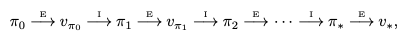
\includegraphics[width=\textwidth]{/chapter4_1}
	\caption{Iterative policy evaluation and improvement}
	\label{fig:policy evaluation}
\end{figure}

\subsection{Value Iteration}
Above, we discussed policy iteration which requires full policy evaluation at each iteration step, an often expensive process which (formally) requires infinite sweeps of the state space to approach the true value function. In value iteration, the policy evaluation is stopped after one visit to each $s \in \mathcal{S}$, or one \textit{sweep} of the state space. Value iteration is achieved by turning the Bellman optimality equation into an update rule:

\begin{equation}
v_{k+1}(s) = \argmax_a \sum_{s',r} p(s', r |s, a)\left[r + \gamma v_k(s')\right]
\end{equation}

for all $s \in \mathcal{S}$. Value iteration effectively combines, in each of its sweeps, one sweep of policy evaluation and one sweep of policy improvement. 

\subsection{Asynchronous Dynamic Programming}
Each of the above methods has required full sweeps of the state space to first evaluate a policy then improve it. Asynchronous dynamic programming does not require us to evaluate the entire state space each sweep. Instead, we can perform in place updates to our value function as they are experienced, focusing only on the most relevant states to our problem initially, then working to less relevant states elsewhere. This can mean that our agent can learn to act well more quickly and save optimality for later.

\subsection{Generalised Policy Iteration}
\begin{figure}[h!]
	\centering
	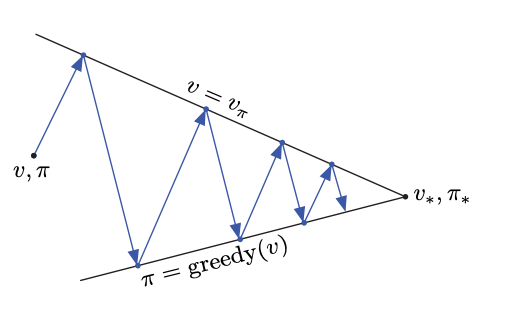
\includegraphics[width=0.5\textwidth]{/chapter4_2}
	\caption{Generalised policy iteration leading to optimality}
	\label{fig:gpi}
\end{figure}

Generalised Policy Iteration is the process of letting policy evaluation and policy improvement interact, independent of granularity. That is to say, improvement/evaluation can be performed by doing complete sweeps of the state space, or it can be performed after every visit to a state (as is the case with value iteration). The level of granularity is independent of our final outcome: convergence to the optimal policy and optimal value function. This process can be illustrated as two convergening lines - Figure \ref{fig:gpi}. We can see that policy improvement and policy evaluation work both in opposition and in cooperation - each time we act greedily we get further away from our true value function; and each time we evaluate our value function our policy is likely no longer greedy. 

\subsection{Key Takeaways}
\begin{itemize}
	\item \textit{Policy evaluation} is the iterative computation of a value function for a given policy. The value function is only truly evaluated in the limit.
	\item \textit{Policy improvement} is the computation of an improved policy given the value function for an existing policy.
	\item By combining the above we achieve \textit{Policy Iteration} and by performing each directly on the value function at each visit to a state we achieve \textit{Value Iteration} - both of which can be used to obtain optimal value functions and policies given complete knowledge of a finite Markov Decision Process.
	\item \textit{Generalised Policy Iteration} is the process of performing policy evaluation and improvement regardless of granularity - leading to convergence to the optimal value functions.
	\item DP methods operate in sweeps through the state space performing an \textit{expected update} operation at each state. These updates are based on expected values at all subsequent states and their probabilities of occurring. In general this idea is known as \textit{bootstrapping}, many RL methods bootstrap to update current beliefs from past beliefs.
\end{itemize}
